\chapter{Neutrinos in the Standard Model and Beyond} \label{chap:theoretical_background}

This chapter introduces the basic properties of neutrinos, their place in the Standard Model of particle physics (SM) and their peculiarities following the description of \cite{Thomson_Particle}.
Section~\ref{sec:neutrino_properties} and Section~\ref{sec:neutrino_interactions} state the general properties of neutrinos and the neutrino-nucleon interactions.
After describing atmospheric neutrinos in Section~\ref{sec:neutrino_atmospheric} the phenomenon of neutrino oscillations is presented in Section~\ref{sec:neutrino_oscillations}.


\section{General Properties} \label{sec:neutrino_properties}

The neutrino is an elementary particle in the SM \cite{Thomson_Particle}.
It belongs to the class of leptons, which itself is a subclass of elementary fermions (spin ${\frac{1}{2}}$ particles).
The fermions - six quarks and six leptons - form the matter content of the universe.
Quarks take part in all three interaction types (forces) of the SM: strong, weak, and electromagnetic (EM) \cite{GLASHOW1961579}.
The charged leptons - electron, muon, and tau - are subject to the weak and the EM interaction.
Neutrinos carry neither electric charge nor color charge and therefore only take part in weak interactions.
There are three distinct neutrino flavors - electron neutrinos, muon neutrinos and tau neutrinos ($\nu_e$, $\nu_{\mu}$, and $\nu_{\tau}$) \cite{PhysRevD.98.030001} - each corresponding to their charged lepton counterparts.

\begin{figure}
	\centering
    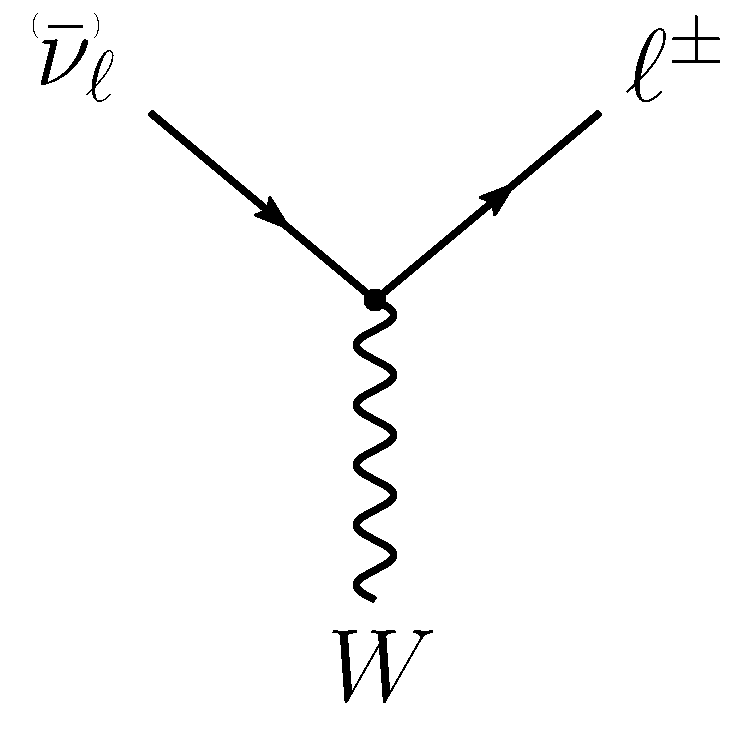
\includegraphics[width=0.25\linewidth]{figures/feynman_CC_nu.pdf}
    \hspace{1cm}
    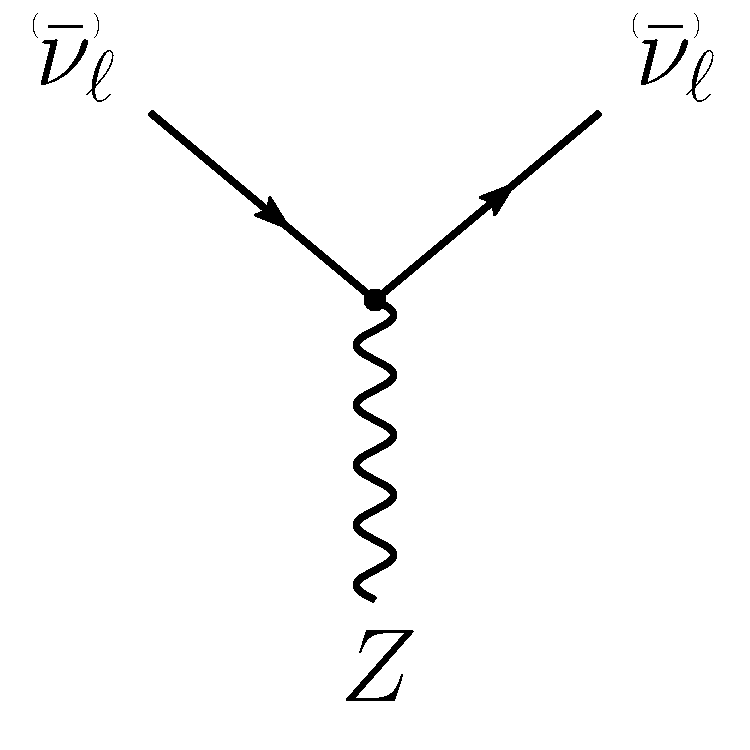
\includegraphics[width=0.25\linewidth]{figures/feynman_NC_nu.pdf}
    \caption[Feynman diagrams of neutrino weak interactions, taken from \cite{ATerliuk}]
    {Feynman diagrams of charged-current (left) and neutral-current (right) neutrino weak interactions. Taken from \cite{ATerliuk}.}
    \label{fig:weak_interactions}
\end{figure}

In the SM, weak interactions are mediated by the three massive bosons $\textbf{W}^+$, $\textbf{W}^-$, and $\textbf{Z}^0$ \cite{Thomson_Particle}.
The large boson masses ($m_{\textbf{W}}\sim80$\,GeV, $m_{\textbf{Z}}\sim90$\,GeV) result in a short range of the force of about $10^{-18}$\,m.
Weak interactions carried by $\textbf{W}^\pm$ bosons are called charged-current (CC) interactions, because charge is transferred between the interacting particles.
In CC interactions, a neutrino is converted into its corresponding charged lepton or vice versa.
Neutral current (NC) interactions are those mediated by $\textbf{Z}^0$ bosons.
Here no charge is transferred.
The Feynman diagrams for CC and NC interactions are shown in Figure~\ref{fig:weak_interactions}.

Although neutrinos are massless in the SM, we know today that they do have a small mass.
The observed phenomenon of neutrino oscillations (see Section~\ref{sec:neutrino_oscillations}) is based on the fact that there is a mass difference between the three neutrino mass eigenstates.
From neutrino oscillation measurements the absolute mass scale cannot be determined, since they only depend on the mass differences, but there are upper limits on the sum of all neutrino masses from cosmological observations.
These upper limits are typically between $0.3$ and $1.3$\,eV \cite{PhysRevD.98.030001}.


\section{Neutrino Interactions} \label{sec:neutrino_interactions}

To describe the neutrino detection principle of IceCube explained in Chapter~\ref{chap:neutrino_detection} we need to understand the weak interaction processes that occur at the energies relevant for this work ($10-100$\,GeV).
The cross-sections are dominated by the following neutrino-nucleon interactions: quasi-elastic scattering (QE), resonant scattering (RES), and deep inelastic scattering (DIS).
The relative importance of the different processes depends on energy as can be seen in Figure~\ref{fig:cross_sections}.

\begin{figure}[ht]
	\centering
    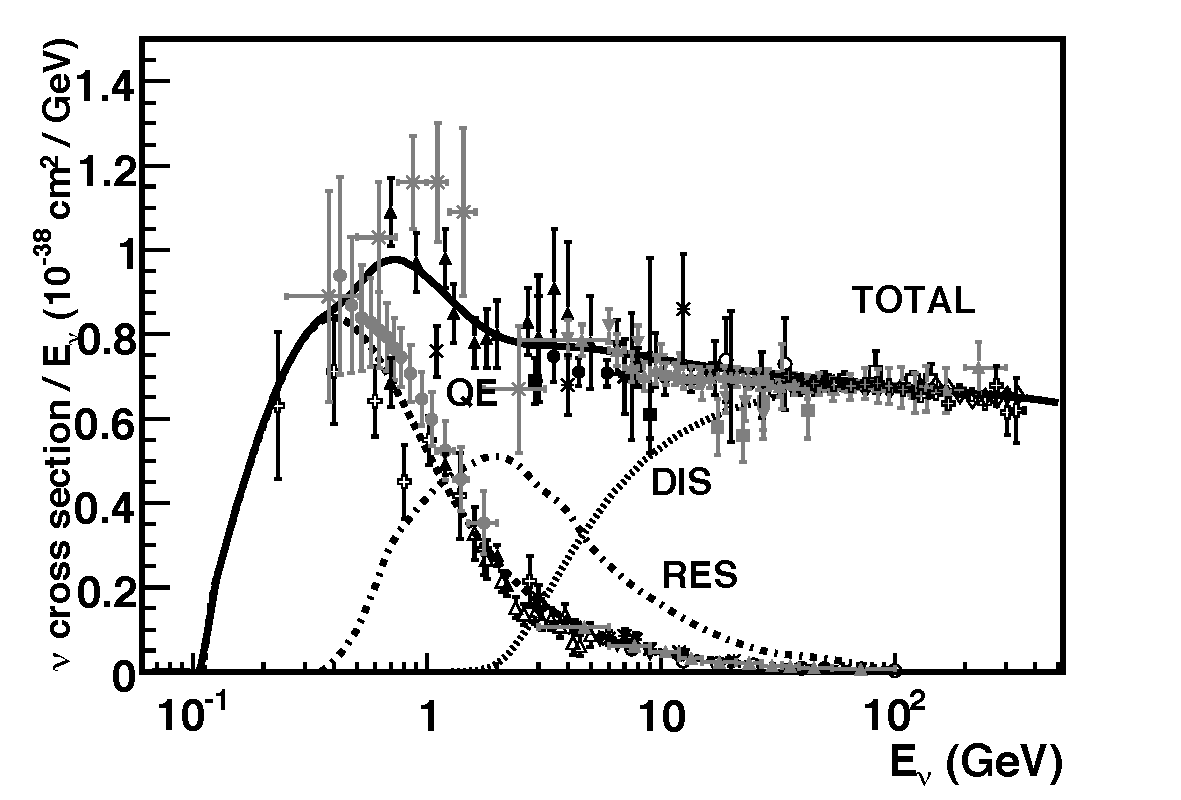
\includegraphics[width=0.495\linewidth]{figures/cc_inclusive_nu.pdf}
    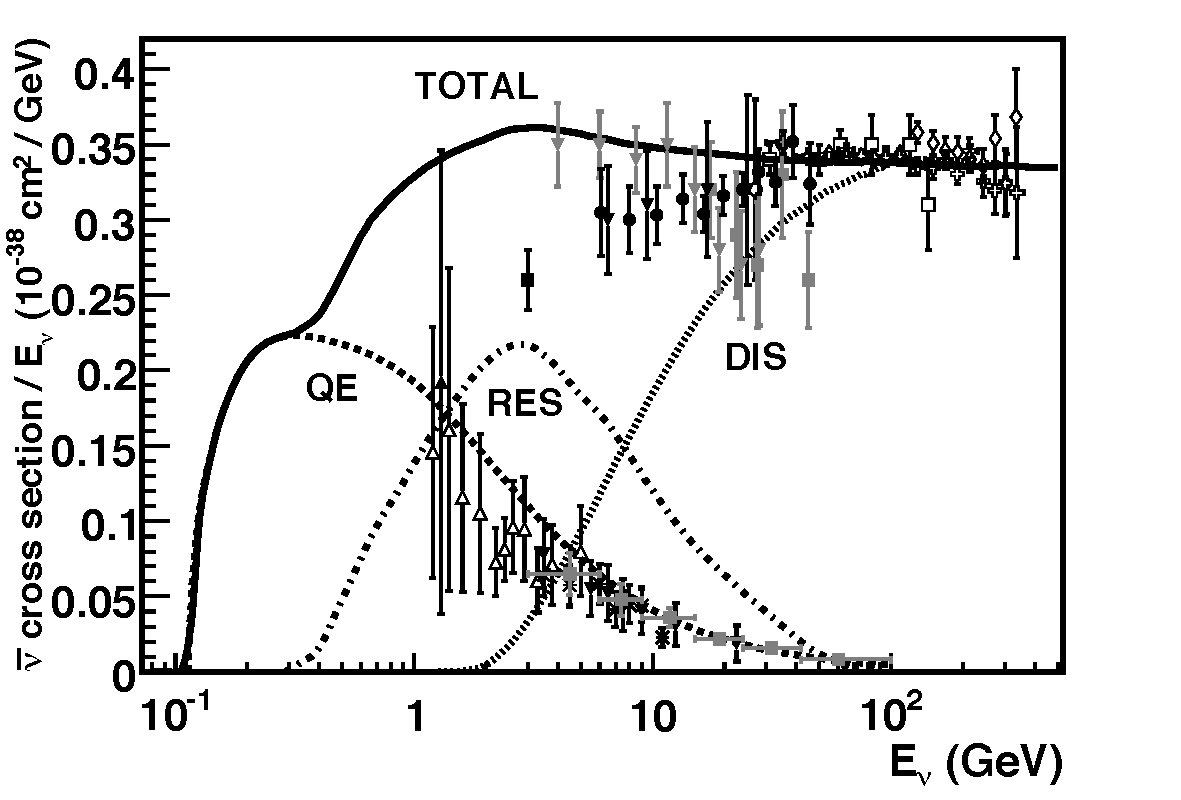
\includegraphics[width=0.495\linewidth]{figures/cc_inclusive_nubar.pdf}
	\caption[Total inclusive neutrino-nucleon cross-sections, taken from \cite{Formaggio_Cross_Sections}.]{Total neutrino(left) and antineutrino(right) per nucleon cross-section divided by neutrino energy plotted against energy.
    The three main scattering processes quasi-elastic scattering (QE), resonant scattering (RES), and deep-inelastic scattering (DIS) are depicted. Taken from \cite{Formaggio_Cross_Sections}.}
    \label{fig:cross_sections}
\end{figure}

An extensive description of all the interactions and the differences between neutrino and antineutrino cross-sections can be found in \cite{Formaggio_Cross_Sections}.
At energies below 5\,GeV, QE and RES occur and the neutrinos interact with approximately point-like protons and neutrons.
The cross-sections of these processes are not linear in energy and the transition region to higher energies is poorly understood.
At higher energies, the interactions are dominated solely by DIS which has a linear dependence on energy above $\sim20\,$GeV.
For a given neutrino energy, it is possible to predict the cross-section in this region.
Here neutrinos interact with a single quark, breaking apart the nucleus and producing a shower of relativistic secondary particles.
Neutrino DIS is the primary detection channel of IceCube.
From Figure~\ref{fig:cross_sections} it can be seen that the interaction cross-sections are very small of the order of $10^{-38}\mathrm{\,cm}^2$.
Because of the small interaction cross-section, very large volume detectors are required to capture a sufficiently large sample of neutrinos to use for precision studies of their properties.
For example, the interaction length of a neutrino with $E_\nu = 10$\,GeV is of $\mathcal{O}(10^{10}\,\mathrm{km})$.

\paragraph{Quasi-elastic scattering (QE)} with nucleons is the main process below 1\,GeV.
Protons are converted to neutrons in antineutrino interactions and vice-versa for neutrino interactions.
Additionally, a charged lepton corresponding to the neutrino/antineutrino flavor is produced.

\paragraph{Resonant scattering (RES)} describes the process of a neutrino scattering off a nucleon producing an excited state of the nucleon in addition to a charged lepton.
RES is the leading process at 1.5-5\,GeV for neutrinos and 1.5-8\,GeV for antineutrinos.

\paragraph{Deep inelastic scattering (DIS)} occurs if a neutrino carries sufficient energy to resolve the underlying structure of the nucleon and interacts with one of the composing quarks.
DIS is the dominant process above 10\,GeV. The nucleon breaks up and a lepton accompanied by a set of hadronic final states is produced.
Whether the lepton is the charged lepton corresponding to the interacting neutrino type, or the neutrino itself depends on the type of DIS interaction.
DIS happens via CC as in 
\begin{equation}
    \begin{split}
        \nu_l + N \rightarrow l^- + X, \\
        \bar{\nu}_l + N \rightarrow l^+ + X, \\
    \end{split}
    \label{eq:dis_cc}
\end{equation}
or NC interactions as
\begin{equation}
    \nu_l + N \rightarrow \nu_l + X.
        \label{eq:dis_nc}
\end{equation}
Here, $X$ stands for any set of final state hadrons and $N$ for the nucleon.
The Feynman diagrams for the processes in Equations~\eqref{eq:dis_cc} and~\eqref{eq:dis_nc} are shown in Figure~\ref{fig:dis_feynman}.

\begin{figure}[h]
    \centering
    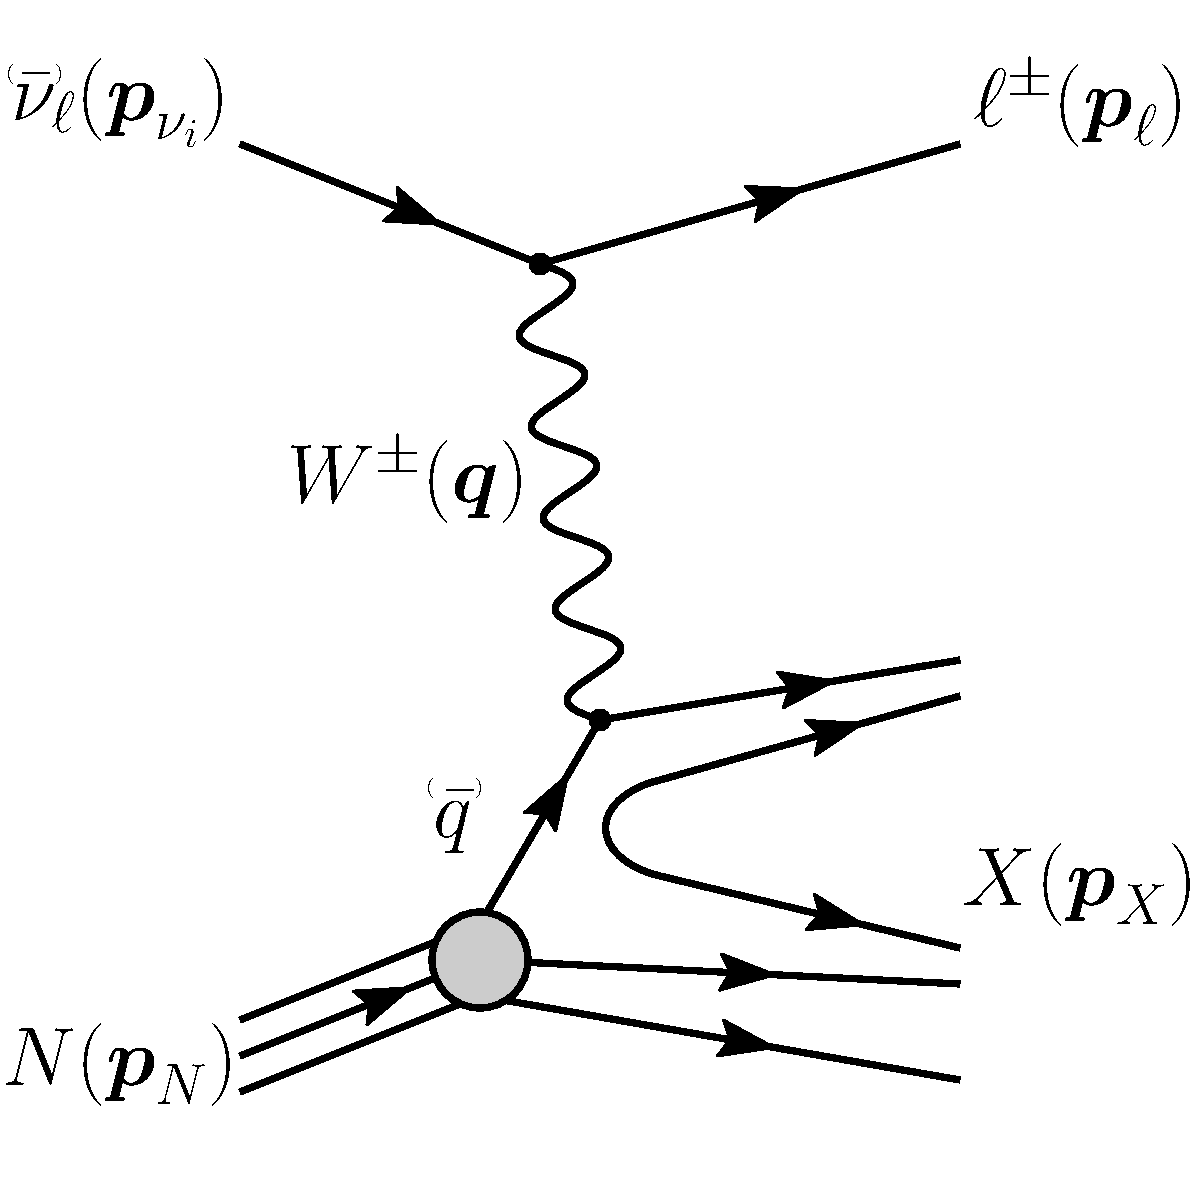
\includegraphics[width=0.4\linewidth]{figures/feynman_DIS_CC_nu_new.pdf}
    \hspace{0.8cm}
    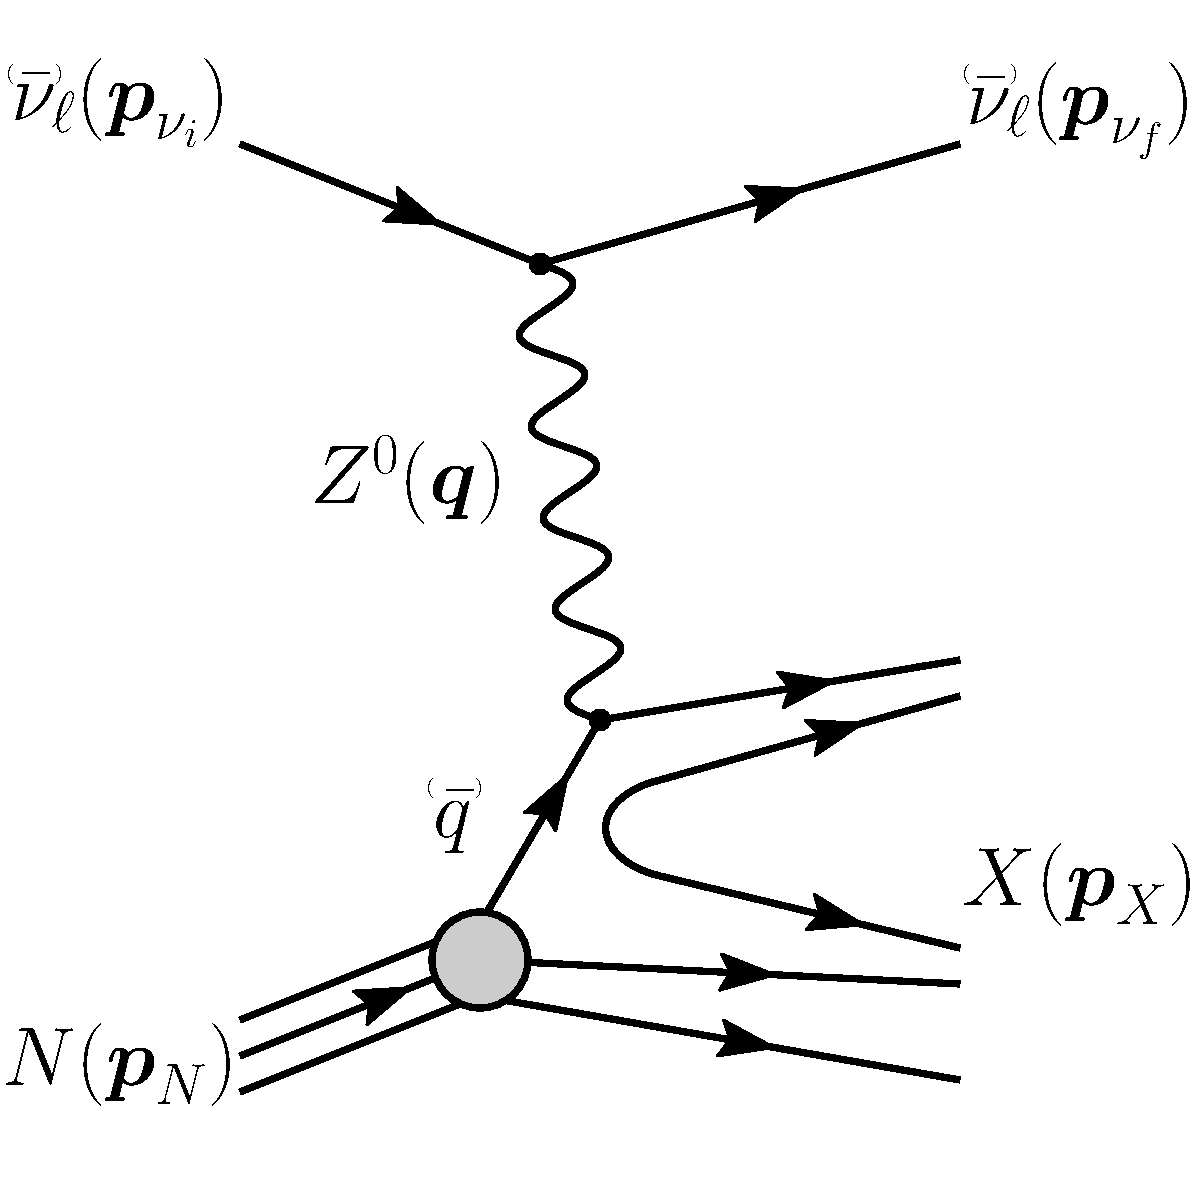
\includegraphics[width=0.4\linewidth]{figures/feynman_DIS_NC_nu_new.pdf}
    \caption[Neutrino-nucleon deep inelastic scattering, taken from \cite{ATerliuk}]{Feynman diagrams for deep inelastic scattering of a neutrino with a nucleon via charged-current (left) and neutral current (right) interactions. Taken from \cite{ATerliuk}.}
    \label{fig:dis_feynman}
\end{figure}


\section{Atmospheric Neutrinos} \label{sec:neutrino_atmospheric}

The flux of neutrinos used for this work exclusively comes from the Earth's atmosphere.
The nominal flux model is calculated by \cite{PhysRevD.92.023004_Honda_Flux} in the energy range of 100\,MeV to 10\,TeV.
When highly relativistic cosmic rays (protons and heavier nuclei \cite{PhysRevD.98.030001}) interact in  the upper atmosphere they produce a shower of particles. 
Neutrinos emerge from the decays of charged pions and kaons ($\pi$ and $K$ mesons) present in these showers.
For energies below 100\,GeV, the leading contribution comes from the pion decay chain
\begin{equation}
    \begin{split}   
        \pi^\pm &\rightarrow \mu^\pm + \nu_\mu(\bar{\nu}_\mu), \\
        \mu^\pm &\rightarrow e^\pm + \bar{\nu}_\mu(\nu_\mu) + \nu_e(\bar{\nu}_e).
    \end{split}
    \label{eq:pion_decay}
\end{equation}
The muons that also originate from this process are considered the main background source for IceCube.
The left part of Figure~\ref{fig:honda_flux} shows the atmospheric neutrino flux for the very broad energy spectrum in which they are produced.
The flux expectations are calculated for the South Pole \cite{PhysRevD.92.023004_Honda_Flux}, where the IceCube detector is located.
From Equation~\eqref{eq:pion_decay} the ratio between muon and electron neutrinos can be inferred to be $N_{\nu_\mu}:N_{\nu_e} \approx 2:1$.
This is only the case at muon energies below 1\,GeV, where all muons decay in flight.
For higher energies, muons can reach earth before decaying increasing the ratio to approximately 10:1 at around 100\,GeV as shown in the right part of Figure~\ref{fig:honda_flux}.
Additionally, kaon decays start to contribute which also increases the number of muons and muon neutrinos.

\begin{figure}[h]
    \centering
    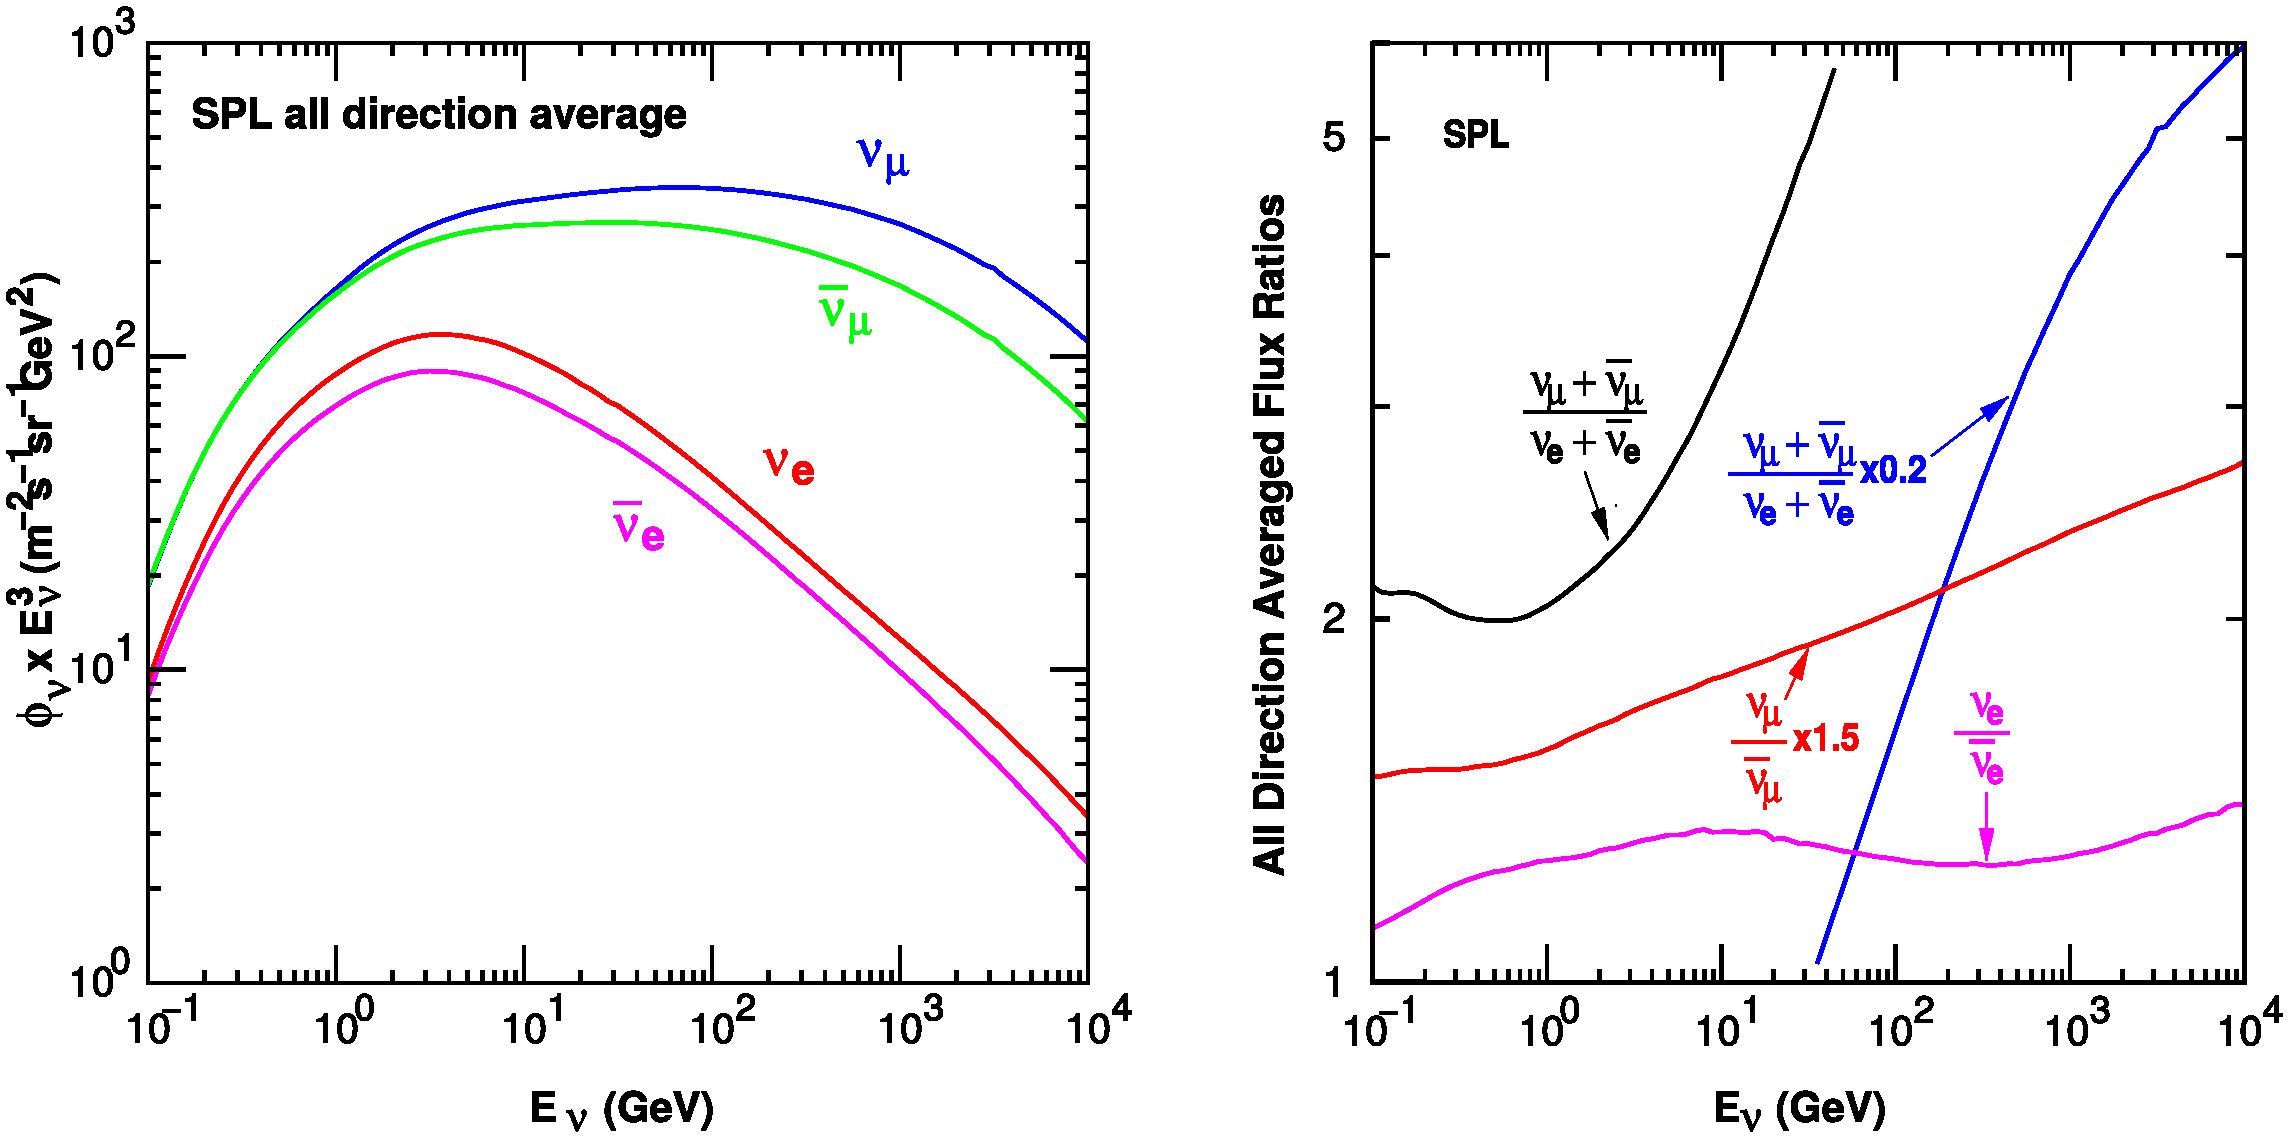
\includegraphics[width=1.0\textwidth]{figures/Honda_alldir-spl_copy.pdf}
    \caption[Atmospheric neutrino fluxes, taken from \cite{PhysRevD.92.023004_Honda_Flux}]{Atmospheric neutrino fluxes of the different flavors as a function of energy (left) and ratios between muon- and electron-neutrinos as well as ratios between neutrinos and antineutrinos for both flavors (right). Calculations are done for the geographic South Pole. Taken from \cite{PhysRevD.92.023004_Honda_Flux}.}
    \label{fig:honda_flux}
\end{figure}

In cosmic ray interactions, charged mesons or tau particles can also be produced, which leads to the formation of tau neutrinos.
However, at the energy range considered for this work, the resulting tau neutrino flux is negligible as compared to the muon neutrino flux \cite{2015EPJWC..9908001F_lepton_fluxes} and is not taken into account.
% is less than 0.1\,\%  of the muon neutrino flux and can, therefore, be neglected.
It should be stated here that there is a rather large uncertainty on the normalization of the atmospheric neutrino flux on the order of 20-30\,\% \cite{PhysRevD.75.043006_neutino_flux_honda} in the energy region of interest.
This is mainly due to uncertainties in the primary cosmic ray spectrum and modeling of the hadronic interactions.


\section{Neutrino Oscillations} \label{sec:neutrino_oscillations}

There are two ways to describe neutrino wave functions based on their Hamiltonian eigenvalues \cite{BILENKY1978225}, as mass eigenstates or as flavor eigenstates.
When applying a plane wave approach to explain the propagation of neutrinos in vacuum, their mass eigenstates evolve as
\begin{equation}
    \ket{\nu_k(t)} = e^{-iE_kt/\hbar}\ket{\nu_k},
    \label{eq:flavor_time_evol}
\end{equation}
where $E_k=\sqrt{\vec{p}^2c^2+m_k^2c^4}$ is the energy of the mass eigenstate $\ket{\nu_k}$, with momentum $\vec{p}$ and mass $m_k$.
Alternatively, they can be described in terms of their flavor eigenstates, which relate the neutrinos to the charged leptons they interact with in weak CC interactions.
The flavor eigenstates are $\nu_e, \nu_\mu$, and $\nu_\tau$, whereas the mass eigenstates are called $\nu_1, \nu_2$, and $\nu_3$ in the standard three-neutrino model.
To understand the propagation of distinct neutrino flavors in time (in vacuum) we need to relate the flavor eigenstates to the mass eigenstates.
For massive neutrinos, each flavor eigenstate is a superposition of mass eigenstates \cite{PhysRevD.98.030001}
\begin{equation}
    \ket{\nu_\alpha} = \sum_kU^*_{\alpha k}\ket{\nu_k},
    \label{eq:neutrino_mixing}
\end{equation}
where $\ket{\nu_\alpha}$ are the weak flavor states with $\alpha=e,\mu,\tau$ and $\ket{\nu_k}$ the mass states with $k=1,2,3$.
$U_{\alpha k}$ is the Pontecorvo-Maki-Nakagawa-Sakata (PMNS) matrix defining the mixing between mass and flavor eigenstates.
The mixing matrix can be parameterized as \cite{PhysRevD.98.030001}
\begin{equation}
    U=\left( 
    \begin{matrix}
        1 & 0 & 0 \\
        0 & c_{23}  & s_{23} \\
        0 & -s_{23} & c_{23} 
    \end{matrix}
    \right) 
    \left( 
    \begin{matrix}
        c_{13} & 0 & s_{13}e^{-i\delta_{CP}} \\
        0 & 1 & 0\\
        -s_{13} e^{i\delta_{CP}} & 0 & c_{13}
    \end{matrix}
    \right ) 
    \left ( 
    \begin{matrix}
        c_{12} & s_{12} & 0 \\
        -s_{12} & c_{12} & 0\\
        0 & 0 & 1
    \end{matrix} 
    \right )  
    \operatorname{diag}(e^{i\rho_{1}},e^{i\rho_{2}},1),
    \label{eq:PMNS_matrix}
\end{equation}
where $c_{ij}=\cos\theta_{ij}$ and $s_{ij}=\sin\theta_{ij}$ are cosine and sine of the mixing angle $\theta_{ij}$, that defines the strength of the mixing between the mass eigenstates i and j and $\delta_{CP}$ is the neutrino CP-violating phase.
Nonzero, non-equal neutrino masses and the neutrino mixing relation in Equation~\eqref{eq:neutrino_mixing} lead to the observed phenomenon of neutrino oscillations.
Oscillation means that a neutrino changes from its initial flavor to another flavor and back after traveling a certain distance.
A produced flavor eigenstate $\ket{\nu_\alpha}$ propagates through space as a superposition of mass eigenstates.
To find the probability that the initial flavor state $\ket{\nu_\alpha}$ ends up as the final flavor state $\ket{\nu_\beta}$ after the time $t$ we calculate
\begin{equation}
    P_{\nu_\alpha \rightarrow \nu_\beta}(t)
    =
    |\braket{\nu_\beta|\nu_\alpha(t)}|^2,
    \label{eq:fermis_golden_rule}
\end{equation}
where $P$ is the probability calculated by applying Fermi's Golden Rule \cite{1927RSPSA.114..243D}.
Fermi's Golden Rule explains the transition rate from one energy eigenstate to another depending on the strength of the coupling between the two.
The strength of the coupling is described by the square of the matrix element.
Using the unitarity of the mixing matrix $U^{-1}=U^\dagger$ to reverse the relation~\eqref{eq:neutrino_mixing} and then time evolve the mass eigenstates with Equation~\eqref{eq:flavor_time_evol} we get the time evolution of the flavor state $\ket{\nu_\alpha(t)}$.
Inserting this result into Equation~\ref{eq:fermis_golden_rule} yields
\begin{equation}
    P_{\nu_\alpha \rightarrow \nu_\beta}(t)
    =
    \sum_{j,k}U^*_{\beta j}U_{\alpha j}U_{\beta k}U^*_{\alpha k}e^{-i(E_k-E_j)t/\hbar},
    \label{eq:probability_raw}
\end{equation}
where the indices $j$ and $k$ run over the mass eigenstates. For small neutrino masses compared to their kinetic energy, we can approximate the energy as
\begin{equation}
    E_k \approx E+\frac{c^4m^2_k}{2E} \hspace{0.25cm} \longrightarrow \hspace{0.25cm} E_k-E_j \approx \frac{c^4\Delta m^2_{kj}}{2E},
\end{equation}
where $\Delta m^2_{kj}=m^2_k-m^2_j$ is the mass-squared splitting between states $k$ and $j$.
If we now replace the time in Equation~\eqref{eq:probability_raw} by the distance traveled by the relativistic neutrinos $t\approx L/c$ we get
\begin{equation}
    \begin{split}
        P_{\nu_\alpha \rightarrow \nu_\beta}(t)
        = 
        \delta_{\alpha \beta}
        -
        4\sum_{j>k}&\textbf{Re}(U^*_{\beta j}U_{\alpha j}U_{\beta k}U^*_{\alpha k})\textrm{sin}^2\Big( \frac{c^3\Delta m^2_{kj}}{4E\hbar}L \Big) \\
        +
        2\sum_{j>k}&\textbf{Im}(U^*_{\beta j}U_{\alpha j}U_{\beta k}U^*_{\alpha k})\textrm{sin}^2\Big( \frac{c^3\Delta m^2_{kj}}{4E\hbar}L \Big),
    \end{split}
    \label{eq:probability_detailed}
\end{equation}
which is referred to as the survival probability if $\alpha=\beta$ and the transition probability if $\alpha\neq\beta$.
The probability in Equation~\ref{eq:probability_detailed} is only nonzero if there are neutrino mass eigenstates with masses greater than zero.
Additionally, there must be a mass-squared difference $\Delta m^2$ and nonzero mixing between the states.
Since we assumed propagation in vacuum in Equation~\ref{eq:flavor_time_evol}, the transition and survival probabilities correspond to vacuum mixing.

\paragraph{Two-neutrino Approximation}

Looking at Equation~\eqref{eq:probability_detailed} it can be noted, that the oscillation frequency for a neutrino with a given energy depends on the mass-squared splitting.
From experiments, we know that the mass splittings $\Delta m^2_{21}$ and $\Delta m^2_{23}$ differ by two orders of magnitude \cite{PhysRevD.98.030001}.
As a result, neutrino oscillation experiments are usually designed to measure at the scale of one of the two mass splittings.
When observing one of the two oscillation frequencies, the other will either be too fast or too slow to be observed.
The oscillations seen in an experiment can, therefore, be described in a simplified two-neutrino scheme, where we only assume two mass eigenstates $\nu_1$, $\nu_2$ that are connected to two flavor eigenstates $\nu_\alpha$, $\nu_\beta$ by the mixing matrix
\begin{equation} 
    U=\left( 
        \begin{matrix}
            \mathrm{cos}\theta & \mathrm{sin}\theta \\
            -\mathrm{sin}\theta & \mathrm{cos}\theta \\
        \end{matrix}
        \right),
    \end{equation}
which is a two-dimensional rotation matrix that depends only on one mixing angle $\theta$ between the two states.
Consequently, the resulting survival/transition probability from Equation~\eqref{eq:probability_detailed} only depends on one mass-squared splitting $\Delta m^2$ and one mixing angle.

\begin{figure}[h]
    \centering
    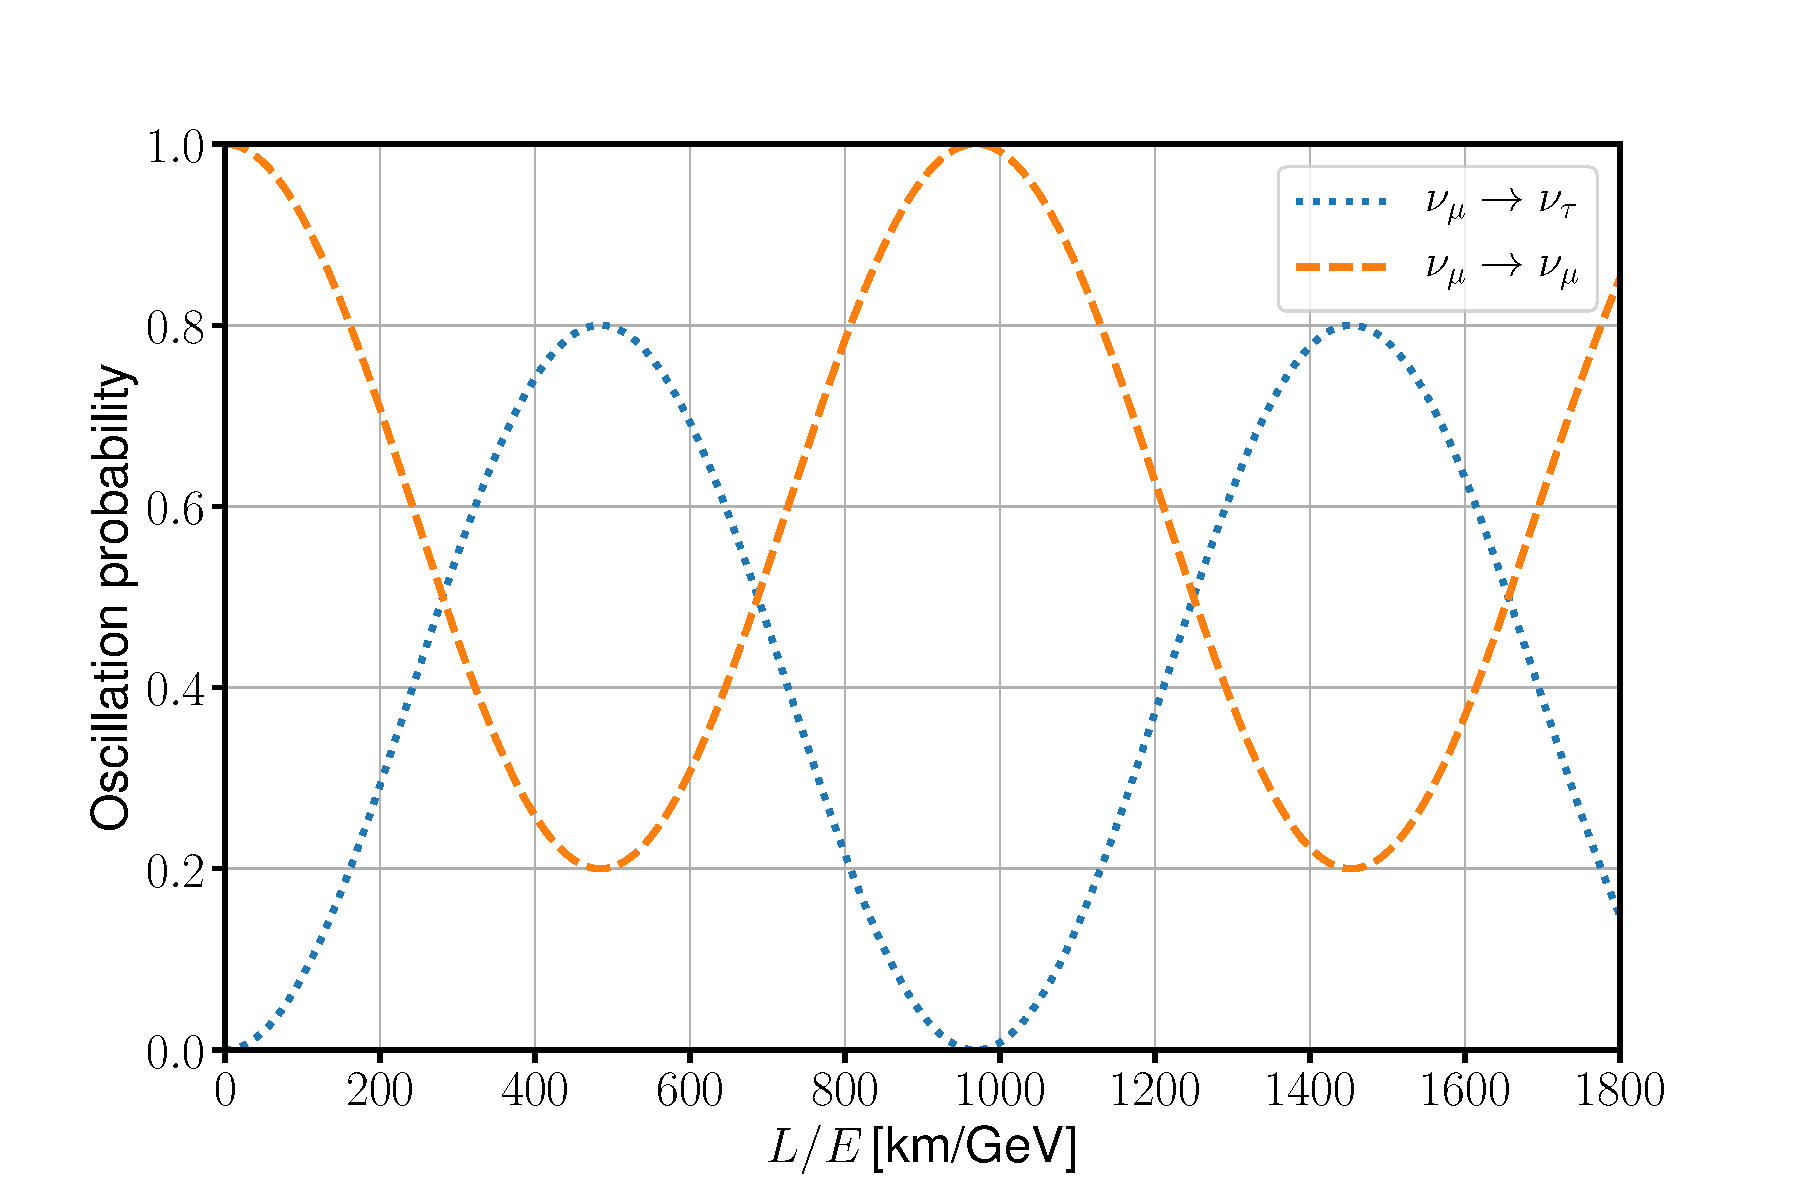
\includegraphics[trim=40 10 60 60, clip, width=0.6\textwidth]{figures/oscillation_probabilities.pdf}
    \caption[Vacuum oscillation probabilities in the two-neutrino approximation]
    {Transition and survival probability for muon neutrinos in the two-neutrino approximation in vacuum (equations \eqref{eq:transition_probability} and~\eqref{eq:survival_probability}) plotted as a function of $L/E$ for $\Delta m^{2}_{32}=2.54\cdot 10^{-3}\,\mathrm{eV}^2$ and $\sin^{2}(\theta_{23}) = 0.8$.}
    \label{fig:oscillation_probabilities}
\end{figure}

DeepCore is sensitive to the fast atmospheric oscillations caused by the bigger mass splitting $\Delta m^2_{23}$, because it is optimized for neutrinos at energies of $\mathcal{O}$(25\,GeV), which have an oscillation length related to $\Delta m^2_{23}$ on the order of the Earth's diameter.
The current global best fit value is $\Delta m^2_{23}=2.54\cdot 10^{-3}\mathrm{eV}^2$ \cite{PhysRevD.98.030001}.
Here the dominant oscillation happens between the flavor states $\nu_\mu$ and $\nu_\tau$.
Formulating the neutrino oscillation phase of Equation~\eqref{eq:probability_detailed} in appropriate units used by the experiment, we get 
\begin{equation}
    \frac{c^3\Delta m^2L}{4E\hbar} \approx 1.267\frac{\Delta m^2\,[\mathrm{eV}^2]\cdot L\,[\mathrm{km}]}{E\,[\mathrm{GeV}]}.
\end{equation}
Inserting this for the two-flavor approximation into the transition probability, we end up with
\begin{equation}
    P_{\nu_\mu \rightarrow \nu_\tau}(L)
    = 
    \textrm{sin}^2(2\theta)\textrm{sin}^2\Big( 1.267 \cdot \frac{\Delta m^2\,[\mathrm{eV}^2]\cdot L\,[\mathrm{km}]}{E\,[\mathrm{GeV}]} \Big),
    \label{eq:transition_probability}
\end{equation}
whereas the survival probability becomes
\begin{equation}
    P_{\nu_\mu \rightarrow \nu_\mu}(L)
    = 1 - P_{\nu_\mu \rightarrow \nu_\tau}(L)
    =
    1 - \textrm{sin}^2(2\theta)\textrm{sin}^2\Big( 1.267 \cdot \frac{\Delta m^2\,[\mathrm{eV}^2]\cdot L\,[\mathrm{km}]}{E\,[\mathrm{GeV}]} \Big).
    \label{eq:survival_probability}
\end{equation}
The transition and survival probability in the two-neutrino approximation are plotted against the traveled neutrino distance divided by the energy in Figure~\ref{fig:oscillation_probabilities}.
The mixing angle in $\sin^{2}(\theta_{23})$ dictates the amplitude of the oscillation while the oscillation length (distance between extrema) is governed by the mass splitting $\Delta m^{2}_{32}$.
